%%%%%%%%%%%%%%%%%%%%%%%%%%%%%%%%%%%%
% 清华大学beamer制作演示文稿模板
% Author: 罗雁天
%%%%%%%%%%%%%%%%%%%%%%%%%%%%%%%%%%%%

% 演示文稿转讲稿请取消注释以下两行
%\documentclass[a4paper]{article} 
%\usepackage{beamerarticle}

% 演示文稿请取消注释以下一行
\documentclass[10pt]{beamer}

% 导入所需要的包
\usepackage{graphicx}
\usepackage{float} 
\usepackage{subfigure}
\setbeamertemplate{caption}[numbered]
\usepackage{multirow}
\usepackage{indentfirst}
%\usepackage[dvipsnames,table,xcdraw]{xcolor}
%\usepackage{beamerarticle}
\usetheme{Berlin}
%\usetheme{Boadilla}
%\usetheme{Hannover}
\useoutertheme[height=1.5cm]{sidebar}
\usecolortheme{spruce}
\usecolortheme{lily}
\usefonttheme{professionalfonts}

%\usepackage{ctex}
\usepackage{xeCJK}
\usepackage{caption}
\setCJKmainfont{KaiTi}
\setmainfont{Times New Roman}
\usepackage{amsmath}
\usepackage{algorithm}
\usepackage{algorithmicx}
\usepackage{algpseudocode}
\usepackage{listings}
%\floatname{algorithm}{算法}
\renewcommand{\algorithmicrequire}{\textbf{输入:}}  
\renewcommand{\algorithmicensure}{\textbf{输出:}}
% 使用bibtex制作参考文献 
\usepackage[backend=bibtex,sorting=none]{biblatex}
\addbibresource{cite.bib} %BibTeX数据文件及位置
\setbeamerfont{footnote}{size=\tiny}
\newcommand{\upcite}[1]{\textsuperscript{\textsuperscript{\cite{#1}}}}
\setbeamertemplate{bibliography item}[text]

% 设置文中代码格式
\lstset{
	columns=fixed,       
	%	numbers=left,                                        % 在左侧显示行号
	numberstyle=\tiny\color{gray},                       % 设定行号格式
	frame=none,                                          % 不显示背景边框
	backgroundcolor=\color[RGB]{245,245,244},            % 设定背景颜色
	keywordstyle=\color[RGB]{40,40,255},                 % 设定关键字颜色
	numberstyle=\footnotesize\color{darkgray},           
	commentstyle=\it\color[RGB]{0,96,96},                % 设置代码注释的格式
	stringstyle=\rmfamily\slshape\color[RGB]{128,0,0},   % 设置字符串格式
	showstringspaces=false,                              % 不显示字符串中的空格
	language=c++,                                        % 设置语言
}

% 设置演示文稿中公式的编号
\makeatletter
\renewcommand \theequation {%
	\ifnum \c@section>\z@ \@arabic\c@section.\fi \ifnum \c@subsection>\z@
	\@arabic\c@subsection.\fi\ifnum \c@subsubsection>\z@
	\@arabic\c@subsubsection.\fi\@arabic\c@equation}
\@addtoreset{equation}{section}
\@addtoreset{equation}{subsection}
\makeatother
\setcounter{section}{-1}

% 设置演示文稿中图片的编号
\renewcommand\thefigure{\thesection.\arabic{figure}}
\makeatletter
\@addtoreset{figure}{section}
\makeatother

\allowdisplaybreaks

% 设置在每一章节前面都显示目录
\AtBeginSection[]{
	\begin{frame}{OUTLINE}
	\tableofcontents[currentsection]
	\end{frame}
}
% 设置在每一小节前面都显示目录
\AtBeginSubsection[]{
	\begin{frame}{OUTLINE}
	\tableofcontents[currentsection,currentsubsection]
    \end{frame}
}
\setlength{\parindent}{2em}
\title{清华大学presentation模板}
\author{\href{mailto:luoyt14thu@gmail.com}{罗雁天 2018310742}}
\date{\today}
\logo{
\includegraphics[height=1.5cm]{Tsinghua2.png}}
%\hyperlinkdocumentend{\logo{
\includegraphics[height=1.5cm]{Tsinghua2.png}}}

\begin{document}
\begin{frame}{清华大学presentation模板}
\titlepage
\end{frame}

\begin{frame}{目录}
\tableofcontents
\end{frame}

\section{简介}

\begin{frame}{简介}
清华大学presentation模板,自己阅读beamer手册制作的模板

\begin{itemize}
	\item 插入图片
	\item 插入表格
	\item 插入公式
	\item 插入代码
	\item 使用参考文献
\end{itemize}
\end{frame}

\section{插入图片}
\begin{frame}{插入图片示例}
只为了模板演示方便,随便插入了一张图片,在使用模板的时候只需要更改图片路径即可。
\begin{figure}[h]
	\centering
	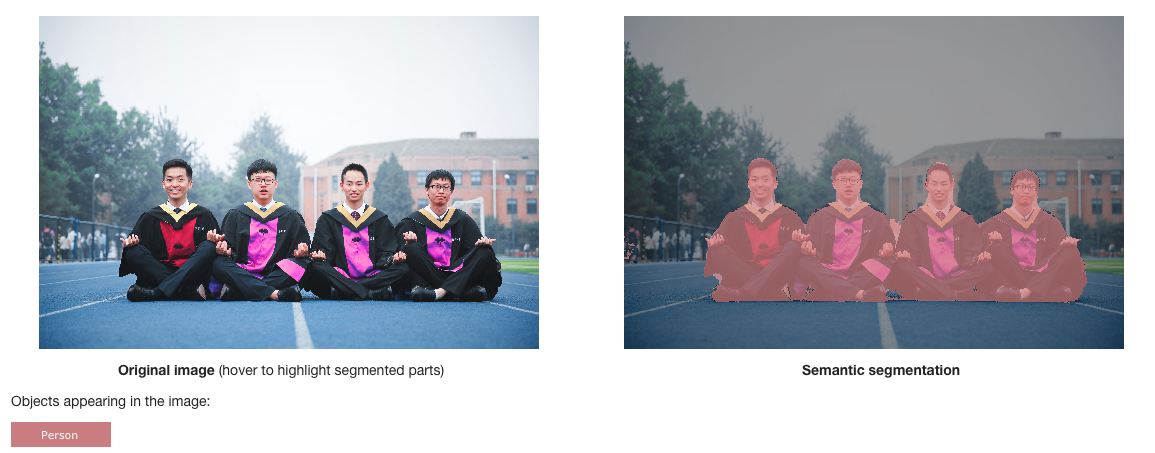
\includegraphics[width=0.9\textwidth]{images/segdemo.png}
	\caption{\label{demo}使用CRF as RNN\upcite{zheng2015conditional}进行图像分割的示例}
\end{figure}
\end{frame}

\section{插入表格}
\begin{frame}{插入表格示例}
\begin{table}
	\centering
	\caption{\label{tab1}插入表格示例}
	\begin{tabular}{|l|c|r|}
	\hline
	操作系统& 发行版& 编辑器\\
	\hline
	Windows & MikTeX & TexMakerX \\
	\hline
	Unix/Linux & teTeX & Kile \\
	\hline
	Mac OS & MacTeX & TeXShop \\
	\hline
	通用& TeX Live & TeXworks \\
	\hline
	\end{tabular}
\end{table}
\end{frame}

\section{插入公式}
\begin{frame}{插入公式示例}
\begin{block}{和差化积公式}
	\begin{equation}
	\label{hecha1}
	\sin x + \sin y = 2\sin \frac{x+y}{2} \cos \frac{x-y}{2}
	\end{equation}
	\begin{equation}
	\label{hecha2}
	\sin x - \sin y = 2\cos \frac{x+y}{2} \sin \frac{x-y}{2}
	\end{equation}
	\begin{equation}
	\label{hecha3}
	\cos x + \cos y = 2\cos \frac{x+y}{2} \cos \frac{x-y}{2}
	\end{equation}
	\begin{equation}
	\label{hecha4}
	\cos x - \cos y = -2\sin \frac{x+y}{2} \sin \frac{x-y}{2}
	\end{equation}
\end{block}
\end{frame}
\section{插入代码}
\begin{frame}[fragile]
\frametitle{插入代码示例}

只为了模板演示方便,写了一段“Hello World!”程序,在使用模板的时候只需要更改代码内容即可。
\begin{lstlisting}
#include <iostream> 
using namespace std; 

int main() { 
    cout << "Hello, World!" << endl;
    return 0;
}
\end{lstlisting}
\end{frame}

\section{使用参考文献}
\begin{frame}[allowframebreaks]{参考文献}
\printbibliography
\end{frame}


\end{document}